\section{Cartes}

Les cartes situent les lieux nommés dans le carnet. Chaque point marque le bourg (sa mairie ou son centre actuels), et non la ferme, la chambre ou le camp d'Hippolyte Combes, qu'on ne peut localiser plus précisément. Le relief est ombré d'après le modèle numérique de terrain Copernicus (résolution de 30~m), avec une exagération verticale qui fait ressortir les vallées de la Somme, de l'Ancre et de l'Hallue ; les cours d'eau viennent de la BD TOPO de l'IGN, les frontières de Natural Earth. Pour les deux cartes à l'échelle de la France (carte générale de la France et carte du chapitre~\textsc{vi}), le relief et les fleuves viennent aussi de Natural Earth. Les lignes de front, schématiques, suivent les localités tenues de part et d'autre, sans le détail des tranchées. Les flèches relient des étapes attestées par le carnet, sans restituer les routes ni les voies ferrées suivies. Les fonds sont actuels : limites, cours d'eau canalisés et bâtiments ne sont pas ceux de 1916.

La première carte situe les principales étapes du carnet, du front aux deux permissions ; la seconde montre le théâtre d'opérations britannique, de la Flandre à la Somme.

\LJpagepaire
\begin{center}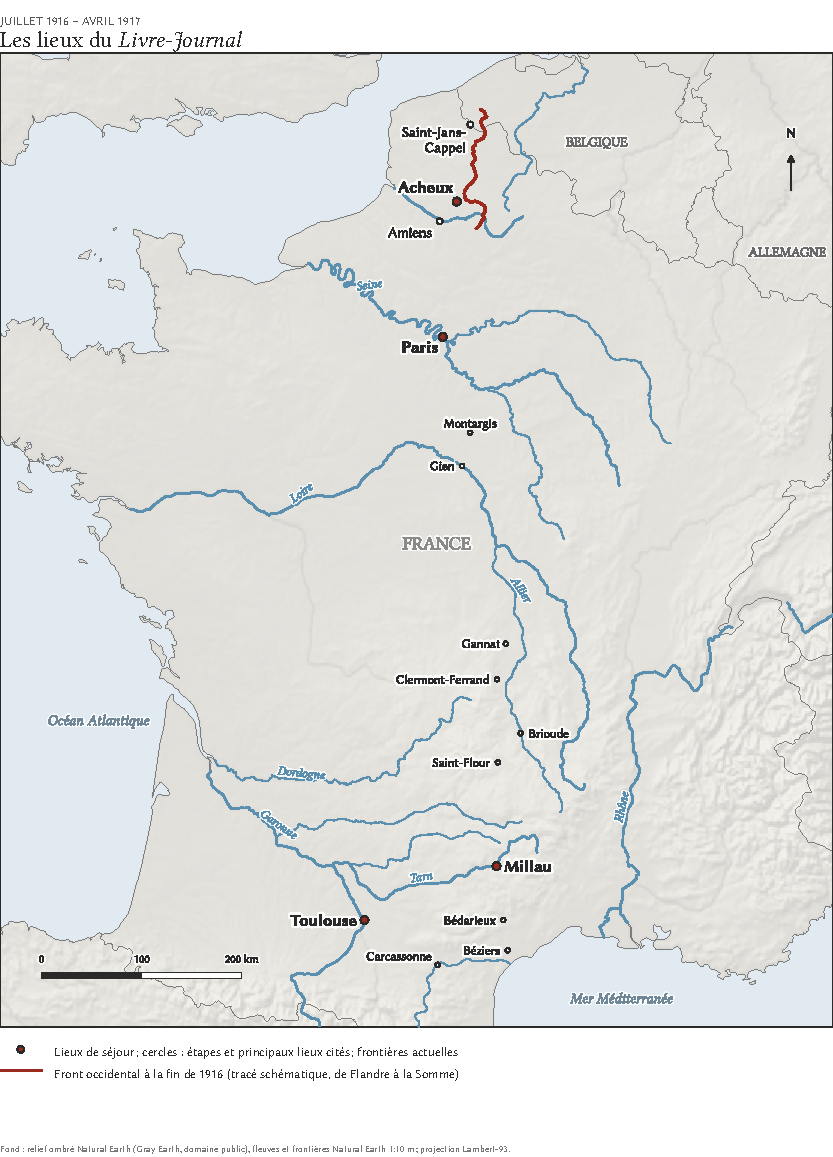
\includegraphics[width=\textwidth]{cartes/pdf/carte_generale_france.pdf}\end{center}
\clearpage
\begin{center}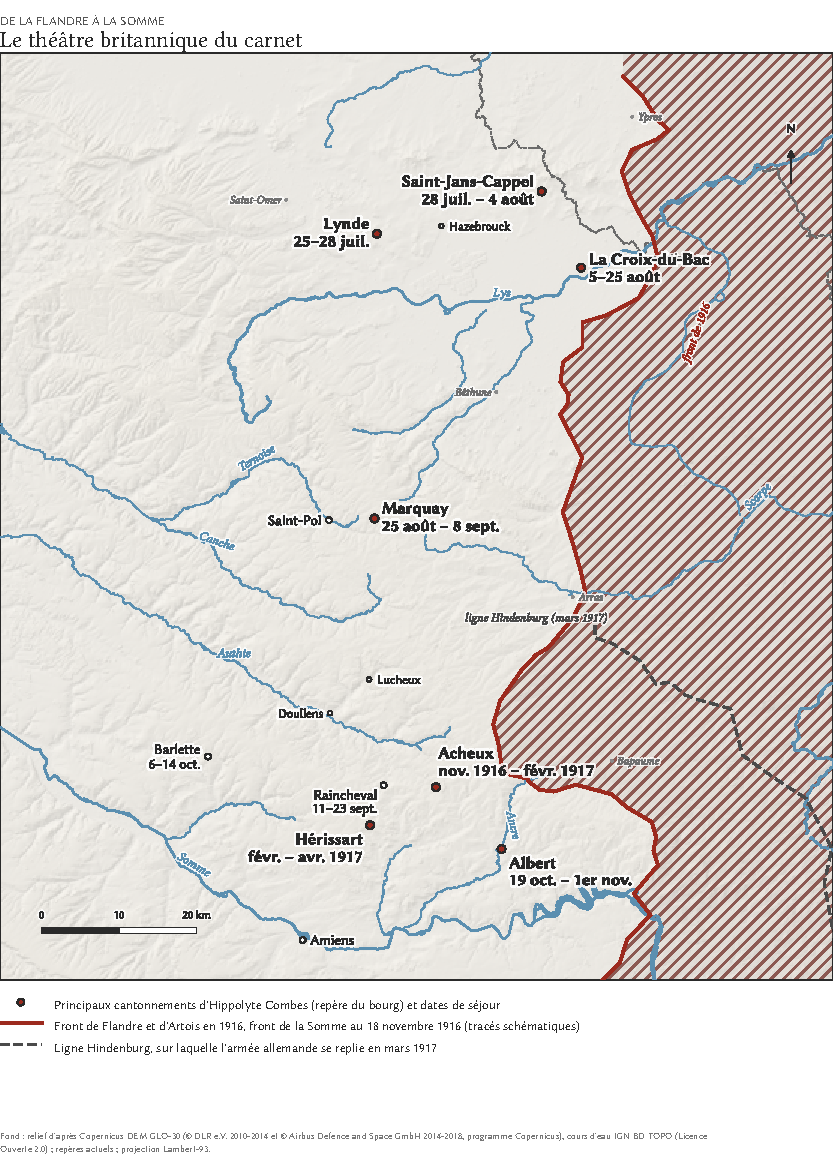
\includegraphics[width=\textwidth]{cartes/pdf/carte_generale_nord.pdf}\end{center}
\clearpage
